\documentclass[a4paper,11pt,fleqn]{article}%fleqn pour aligner les equations à gauche
\usepackage{../../Styles/Cours}

\newcommand{\chnum}{Chapitre 18}
\newcommand{\chtitle}{Interférences et diffraction}
\newcommand{\dtype}{Cours}


\begin{document}
\maketitle

\section{Diffraction}
	\subsection{Définition}
	Toutes les ondes, mécaniques ou électromagnétiques peuvent subir le phénomène de diffraction.\\
	La diffraction est une propriété des ondes qui se manifeste par un changement des direction de propagation de l'onde, lorsque celle-ci rencontre un obstacle ou une ouverture.
	\subsection{Conditions d'observation}
	La phénomène de diffraction est observé si l'onde rencontre un obstacle ou une ouverture de dimension comparable ou inférieure à sa longueur d'onde.
	\subsection{Angle caractéristique de diffraction}
	Le phénomène de diffraction ne modifie ni la longueur d'onde, ni la fréquence de l'onde. Il est caractérisé par un angle noté $\theta$ (thêta). Dans le cas d'une onde progressive périodique :
	$$\theta = \dfrac{\lambda}{a}$$
	\begin{center}
	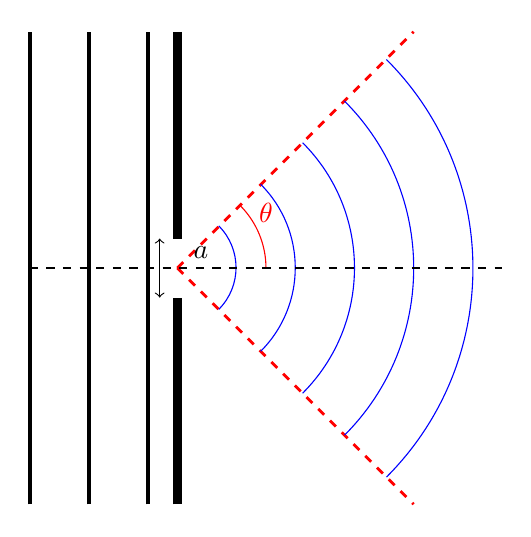
\begin{tikzpicture} [scale=.75]%onde eau
\foreach \k in {0,...,2} {
\draw [line width = 1.5pt](\k,-4) --(\k,4);}

\draw [line width = 3pt](2.5,-4) --(2.5,-.5);
\draw [line width = 3pt](2.5,4) --(2.5,.5);
\draw [line width = 1pt,red,dashed](2.5,0) --(6.5,4);
\draw [line width = 1pt,red,dashed](2.5,0) --(6.5,-4);

\draw [blue] (3.2, -.7) arc (-45:45:1 );
\draw [blue] (3.91, -1.41) arc (-45:45:2 );
\draw [blue] (4.62, -2.12) arc (-45:45:3 );
\draw [blue] (5.33, -2.83) arc (-45:45:4 );
\draw [blue] (6.04, -3.54) arc (-45:45:5 );

\draw [red] (4, 0) arc (0:45:1.5 );
\draw [red] (4,.6) node[above]{$\theta$};
\draw [dashed] (0,0) -- (8,0 );

\draw [<->] (2.2,-.5) to (2.2,.5);
\node (a) at (7,0){};
\draw (2.9,0) node[above]{$a$};
\end{tikzpicture}
\hspace{1.2cm}
\begin{tikzpicture}[scale=.75]
\fill [red!40] (10,0)ellipse(0.2 and 1);
\fill [red!40] (10,2)ellipse(0.2 and .5);
\fill [red!40] (10,-2)ellipse(0.2 and .5);

\fill [red] (0,-.5) -- (0,.5) --(2,.5) --(2,-.5) -- cycle;
\draw [line width = 1.5pt] (2,.5) -- (2,2.5);
\draw [line width = 1.5pt] (2,-.5)--(2,-2.5);

\draw [<->] (2.5,-.5) to (2.5,.5);
\draw (2.5,.5) node[above right]{$a$};

\draw [dashed] (2,0) -- (10,0);
\draw [dashed] (2,0) -- (10, 1);
\draw [dashed] (2,0) -- (10, -1);
\draw (10,-3) -- (10,3);

\draw [<->] (2,-2.5) to (10,-2.5);
\draw (6,-2.5) node[below]{$D$};

\draw (7,0) arc(0:18:2);
\draw (7.5,-.7) arc(-5:15:2);

\draw (7,.3) node[right]{$\theta$};
\draw (7.5,-.35) node[right]{$\theta$};

\fill [red!40] (10,0)ellipse(0.2 and 1);
\fill [red!40] (10,2)ellipse(0.2 and .5);
\fill [red!40] (10,-2)ellipse(0.2 and .5);

\draw [->] (11,1) to (10.3,.5);
\draw (11,1) node[right]{Tache centrale};

\draw [<->] (10.5,-1) to (10.5,0);
\draw (11,-.5) node[right]{$\dfrac{L}{2}$};
\end{tikzpicture}
	\end{center}


\section{Interférences à deux ondes}
	\subsection{Définition}
	Il s'agit d'une propriété des ondes qui se caractérise en tout point d'un milieu par la superposition de deux ondes de même nature et de même fréquence. Pour cela, les ondes qui interfèrent doivent être émises par deux sources cohérentes. On dit que deux sources sont cohérentes si elles émettent des ondes de même fréquence et avec un déphasage constant.\\
	\begin{minipage}{.35\textwidth}
	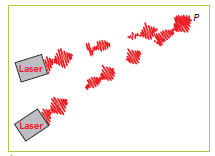
\includegraphics[scale=.8]{Ressources/TSPE_C9_Cours_Fig4.png}
	\end{minipage}
	\begin{minipage}{.6\textwidth}
	\begin{small}
	Sur l'image ci-contre, on observe des trains d'ondes émis de façon aléatoire pour deux sources lumineuses. Même si les ondes sont de même fréquence, leur déphasage n'est pas constant (le déphasage en un point $P$ donné n'est pas toujours le même). Le phénomène d'interférence ne peut pas être observé.
	\end{small}
\end{minipage}
	\subsection{Étude du phénomène (cas d'ondes à la surface de l'eau)}
	\begin{minipage}{.48\textwidth}
	\begin{center} 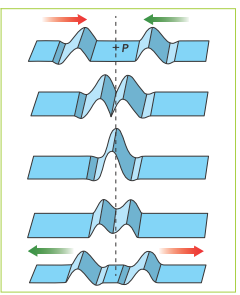
\includegraphics[scale=.6]{Ressources/TSPE_C9_Cours_Fig1.png}\end{center}
	L'image ci-dessus illustre le croisement de deux ondes à la surface de l'eau. On observe que \textbf{lorsque les deux ondes se superposent, leurs élongations s'ajoutent}.
	\end{minipage}
	\hspace{.2cm}
	\begin{minipage}{.48\textwidth}
	\begin{center} 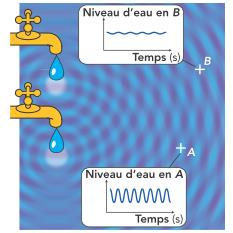
\includegraphics[scale=.7]{Ressources/TSPE_C9_Cours_Fig2.png}\end{center}
	Sur cette nouvelle image, on observe la superposition de deux ondes circulaire créées par deux sources périodiques de même fréquence.
	\end{minipage}
		\subsubsection*{Au point A :}
		Les deux signaux coïncident (maxima au même instant et minima au même instant). Les deux signaux sont \textbf{en phase}. L'amplitude de l'onde résultante est la somme des amplitudes des deux ondes. Cette somme est plus grande que chacune des deux ondes. Les \textbf{interférences sont dites constructives}.
		\noindent
\begin{center}
\begin{minipage}{8cm}
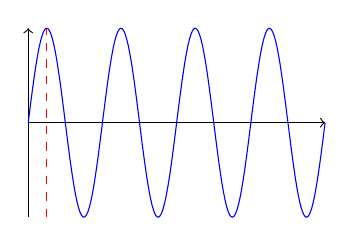
\begin{tikzpicture}[scale=.6]
%\draw (-3*pi,-2) grid (-pi,2);
\draw [->](-3*pi,0) to (-pi,0);
\draw [->](-3*pi,-2) to (-3*pi,2);
\draw [dashed, color = red] (-3*pi+pi/8, -2) -- (-3*pi+pi/8, 2);
\draw [domain=-3*pi:-pi, samples = 200, color = blue] plot (\x, {2*sin{\x*4 r}});
\end{tikzpicture}\\
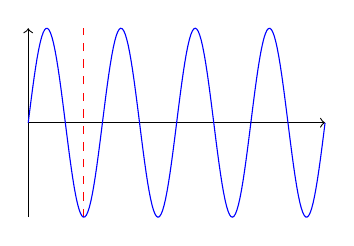
\begin{tikzpicture}[scale=.6]
\draw [->](-3*pi,0) to (-pi,0);
\draw [->](-3*pi,-2) to (-3*pi,2);
\draw [dashed, color = red] (-3*pi+3*pi/8, -2) -- (-3*pi+3*pi/8, 2);
\draw [domain=-3*pi:-pi, samples = 200, color = blue] plot (\x, {2*sin{\x*4 r}});
\end{tikzpicture}
\end{minipage}
\begin{minipage}{8cm}
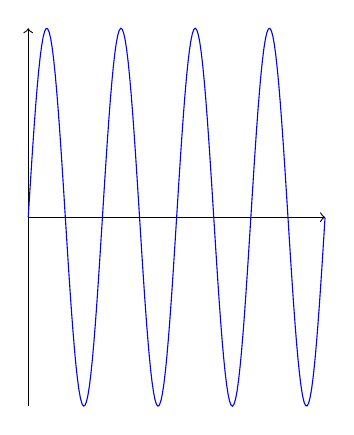
\begin{tikzpicture}[scale=.6]
\draw [->](-3*pi,0) to (-pi,0);
\draw [->](-3*pi,-4) to (-3*pi,4);
\draw [domain=-3*pi:-pi, samples = 200, color = blue] plot (\x, {2*sin{\x*4 r} + 2*sin{\x*4 r}});
\end{tikzpicture}
\end{minipage}
\end{center}
		\subsubsection*{Au point B :}
		Pour un même instant, les maxima d'un signal coïncident avec les minima de l'autre signal. \textbf{Les ondes sont dit en opposition de phase}.\\
		L'amplitude de l'onde résultante est la comme des amplitudes des deux ondes. Cette somme est plus petite que chacune des deux ondes, voire nulle. \textbf{Les interférences sont destructives}.\\
		\noindent
\begin{center}
\begin{minipage}{8cm}
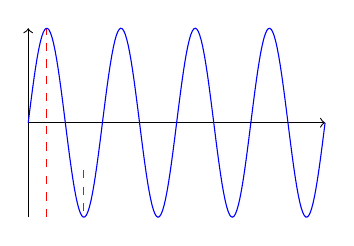
\begin{tikzpicture}[scale=.6]
\draw [->](-3*pi,0) to (-pi,0);
\draw [->](-3*pi,-2) to (-3*pi,2);
\draw [dashed, color = red] (-3*pi+pi/8, -2) -- (-3*pi+pi/8, 2);
\draw [dashed, color = red] (-3*pi+3*pi/8, -1) -- (-3*pi+3*pi/8, -2);
\draw [domain=-3*pi:-pi, samples = 200, color = blue] plot (\x, {2*sin{\x*4 r}});
\end{tikzpicture}\\
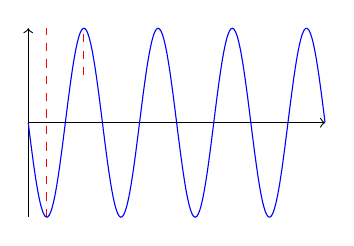
\begin{tikzpicture}[scale=.6]
\draw [->](-2.75*pi,0) to (-.75*pi,0);
\draw [->](-2.75*pi,-2) to (-2.75*pi,2);
\draw [dashed, color = red] (-2.5*pi-pi/8, -2) -- (-2.5*pi-pi/8, 2);
\draw [dashed, color = red] (-2.5*pi+pi/8, 1) -- (-2.5*pi+pi/8, 2);
\draw [domain=-2.75*pi:-.75*pi, samples = 200, color = blue] plot (\x, {2*sin{\x*4 r}});
\end{tikzpicture}
\end{minipage}
\begin{minipage}{8cm}
\begin{tikzpicture}[scale=.6]
\draw [->](-3*pi,0) to (-pi,0);
\draw [->](-3*pi,-4) to (-3*pi,4);
\draw [domain=-3*pi:-pi, samples = 200, color = blue] plot (\x, {2*sin{\x*4 r} - 2*sin{\x*4 r}});
\end{tikzpicture}
\end{minipage}
\end{center}
		\subsubsection*{À tout autre point du milieu :}
		On observe des vibrations d'amplitude intermédiaire.\\
	Les points du milieu de propagation où les interférences sont constructives (ou destructives) sont positionnés de manière régulière et précise.\\
	Soient les deux sources cohérentes $S_1$ et $S_2$ et un point $M$ du milieu comme ci-contre.\\
	Le caractère constructif ou destructif de la superposition des deux ondes en un point $M$ dépend du retard d'une onde par rapport à l'autre ou, ce qui est équivalent, à la différence de trajet entre les deux ondes, appelée \textbf{différence de chemin} et notée $\delta$ (delta).
		$$\delta = d_2 - d_1 = S_2M - S_1M $$
	\begin{itemize}
	\item Les interférences sont \textbf{constructives} quand les ondes arrivent \textbf{en phase} au point $M$.\\ Dans ce cas : $\delta = k\cdot \lambda$ avec $k$ un entier relatif appelé ordre d'interférences.
	\item Les interférences sont \textbf{destructives} quand les ondes arrivent \textbf{en opposition de phase} au point $M$. \\ Dans ce cas : $\delta = \lambda \cdot \left( k+\dfrac{1}{2} \right)$
	\end{itemize}
\begin{center}
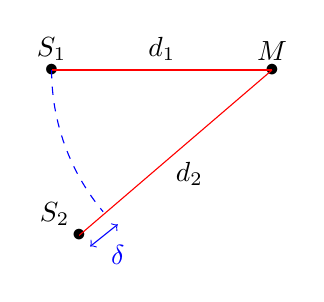
\begin{tikzpicture}[scale=.7]
\node (S1) at (0,0){};
\draw (S1) node{$\bullet$} node[above]{$S_1$};
\node (M) at (4,0){};
\draw (M) node{$\bullet$} node[above]{$M$};
\node (S2) at (.5,-3){};
\draw (S2) node{$\bullet$} node[above left]{$S_2$};
\draw [color = red](0,0) -- (4,0);
\draw [color = red] (.5,-3) -- (4,0);
\draw [dashed,blue] (0,0) arc (180:220:4);
\node (I) at (1,-2.6){};
\draw [<->,blue] (.7,-3.2) to (1.2,-2.8);
\draw [blue] (1.2,-3) node[below]{$\delta$};
\draw (2,0) node[above]{$d_1$};
\draw (2.5,-1.5) node[below]{$d_2$};
\end{tikzpicture}
\end{center}


\section{Interférence de deux ondes lumineuses monochromatiques}
	\subsection{Expérience des trous d'Young}
	Pour observer une figure d'interférences stable avec de la lumière, il faut créer deux sources secondaires à partir d'une source unique. \textbf{C'est la seule manière d'obtenir des sources cohérentes}.\\
	On peut par exemple utiliser le dispositif des fentes d'Young ou celui des trous d'Young.\\
	
\begin{center}
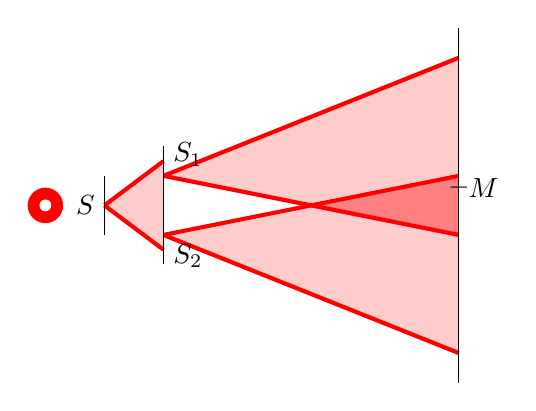
\begin{tikzpicture}[scale=.75]
\fill [red] (0,0) circle (.3) ;
\fill [white] (0,0) circle (.1) ;


\fill[color = red!20](1,0) -- (2,.75) -- (2,-.75) --cycle;
\fill[color = red!20](2,.5) -- (7,2.5) -- (7,-.5) --cycle;
\fill[color = red!20](2,-.5) -- (7,.5) -- (7,-2.5) --cycle;
\fill[color = red!50](4.5,0) -- (7,.5) -- (7,-.5) --cycle;

\draw [line width = 1.5pt,red](1,0) --(2,.75);
\draw [line width = 1.5pt,red](1,0) --(2,-.75);

\draw [line width = 1.5pt,red](2,.5) --(7,2.5);
\draw [line width = 1.5pt,red](2,.5) --(7,-.5);

\draw [line width = 1.5pt,red](2,-.5) --(7,.5);
\draw [line width = 1.5pt,red](2,-.5) --(7,-2.5);

\draw (1,-.5) -- (1,.5);
\draw (2,-1) -- (2,1);
\draw (7,-3) -- (7,3);
\draw (1,0) node[left]{$S$};
\draw (2,.5) node[above right]{$S_1$};
\draw (2,-.5) node[below right]{$S_2$};
\draw (7,.3) node{$-$} node[right]{$M$};
\end{tikzpicture}
\end{center}
	Sur un écran, on observe à la fois les phénomènes de diffraction et d'interférences.\\
	\begin{center}
	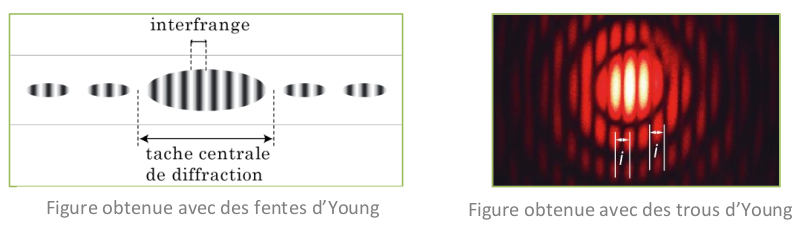
\includegraphics[scale=.5]{Ressources/TSPE_C9_Cours_Fig5.png}
	\end{center}	 
	
	\subsection{Conditions d'interférences constructives ou destructives}
	Les lieux d'interférences constructives (franges brillantes) et destructives (franges sombres) sont fonction de la différence de trajet de deux ondes. Dans le cas des deux ondes lumineuses, la différence de trajet est appelée \textbf{différence de chemin optique $\delta$} et dépend de l'indice optique $n$ du milieu traversé. On a :
	\begin{eqnarray}
	\delta = n \cdot S_2M - n\cdot S_1M = n \cdot (S_2M - S_1M) \nonumber
	\end{eqnarray}
	\begin{itemize}
		\item On observe des interférences \textbf{constructives} (franges brillantes) lorsque les ondes arrivent \textbf{en phase} au point $M$, c'est-à-dire lorsque : $\delta = l \cdot \lambda_0$ avec $k$ un entier relatif et $\lambda_0$ la longueur d'onde dans le vide.
		\item On observe des interférences \textbf{destructives} (franges sombres) lorsque les ondes arrivent en \textbf{opposition de phase} au point $M$, c'est-à-dire lorsque $\delta = \lambda_0 \cdot \left(k + \dfrac{1}{2} \right)$
	\end{itemize}
	
	\subsection{Interfrange}
	La distance qui sépare les milieux de deux franges brillante consécutives (ou de deux franges sombres consécutives) est appelé \textbf{interfrange}, $i$.\\
	Dans le vide ou l'air, $i = \dfrac{\lambda \cdot D}{a}$\\
	avec $a$ la distance entre les deux fentes et $D$ la distance fentes-écran.


















\end{document}